\documentclass[a4paper, 14pt]{extarticle}
\usepackage{indentfirst}
\usepackage[T2A]{fontenc}
\usepackage[utf8]{inputenc}
\usepackage[english, russian]{babel}
\usepackage{amsmath, amssymb, amsthm, amscd, latexsym}
\usepackage[nottoc,numbib]{tocbibind}
\usepackage{graphicx, caption}
\usepackage[left=3cm,right=2cm,top=2cm,bottom=3cm]{geometry}
\setlength{\parindent}{1.25cm}
\linespread{1.25}
\graphicspath{{pictures/}}

\newtheorem{theorem}{Теорема}[subsection]
%\numberwithin{theorem}{subsection}
\newtheorem{lemma}{Лемма}
\newtheorem{corollary}{Следствие}
\newtheorem{proposition}{Предложение}
\newtheorem{assertion}{Утверждение}
\theoremstyle{definition}
\newtheorem{definition}{Определение}[subsection]
%\numberwithin{definition}{subsection}
\newtheorem{remark}{Замечание}
\newtheorem{example}{Пример}
\renewcommand{\thetheorem}{\arabic{theorem}}
\renewcommand{\thedefinition}{\arabic{definition}}

\usepackage{hyperref}
\hypersetup{
    colorlinks=true,
    linkcolor=blue,
    filecolor=magenta,
    urlcolor=black,
    pdfpagemode=FullScreen,
}


\title{EM-algorithm}
\author{Р.\,С.~Мурадасилов}
\date{2020}

\begin{document}
\begin{titlepage}
\begin{center}
        
\textbf{Филиал Московского Государственного Университета\\
имени М.В. Ломоносова в г. Ташкенте} \vskip 0.3cm
\textbf{Факультет прикладной математики и информатики} \vskip 0.3cm
\textbf{Кафедра прикладной математики и информатики} \vskip 3cm
            
\textbf{Мурадасилов Руслан Серверович} \vskip 1cm
            
\textbf{ВЫПУСКНАЯ КВАЛИФИКАЦИОННАЯ РАБОТА} \vskip 1cm
            
\normalsize { \textbf{на тему: \guillemotleft EM-алгоритм и его применение в статистических задачах\guillemotright \\ \vskip 0.5cm
по направлению 01.03.02 \guillemotleft Прикладная математика и информатика\guillemotright} }
\vskip 1.5cm
\end{center}

\begin{flushleft}
ВКР рассмотрена и рекомендована к защите \vskip 5pt
зав. кафедрой \guillemotleftПМиИ\guillemotright, к.ф.-м.н., доцент\rule{3.2cm}{0.5pt} Строгалов А.\,С.
\end{flushleft}
\begin{flushleft}
Научный руководитель:\vskip 5pt
д.ф.-м.н., профессор \rule{6.9cm}{0.5pt} Абдушукуров А.\,А.
\end{flushleft}
          
\begin{flushright}
<<\rule{1cm}{0.5pt}>>\rule{3.5cm}{0.5pt} 2021 г.
\end{flushright}
        
\vfill   
\begin{center}
Ташкент 2021
\end{center}
\end{titlepage}

\begin{abstract}
    В данной работе рассматривается EM-алгоритм и его применение в статистических задачах.
    
    В первой части работы описан сам EM-алгоритм, его свойства и модификации. Вторая часть работы представляет собой исследование по применению EM-алгоритма к цензурированной выборке на языке программирования Python с помощью модуля GaussianMixture библиотеки Scikit-Learn и модуля Stats библиотеки SciPy.
    
    \textbf{Ключевые слова}: цензурированная выборка, EM-алгоритм, \\ 
    GaussianMixture
\end{abstract}

\selectlanguage{english}

\begin{abstract}
    This paper is devoted to EM-algorithm and its application in statistical problems.
    
    The first part of the paper describes EM-algorithm, its properties and modifications. The second part of the paper represents a research on application of EM-algorithm to censored data on Python programming language using the GaussianMixture module of Scikit-Learn library and Stats module of SciPy library.
    
    \textbf{Keywords}: censored data, EM-algorithm, GaussianMixture
\end{abstract}

\selectlanguage{russian}

\setcounter{page}{2}
\newpage

\tableofcontents
\newpage

\section{Введение}
EM-алгоритм в математической статистике используется для нахождения оценок максимального правдоподобия параметров вероятностной модели, в случае, когда модель зависит от некоторых скрытых данных. Как правило, EM-алгоритм применяется при решении задач двух типов.

К первому типу относятся задачи с \emph{действительно} неполными данными, когда некоторые статистические данные отсутствуют в силу каких-либо причин. Ко второму же типу можно отнести задачи, в которых удобно вводить скрытые переменные для упрощения подсчета функции правдоподобия. Примером такой задачи может служить кластеризация.

В данной работе приведено описание EM-алгоритма и его свойства, а также предложен пример с его применением к задаче первого типа.

В первой части работы дан теоретический материал, в котором подробно изложены E-шаг и M-шаг в общем случае, а также на примере разделения смеси нормальных распределений.

Вторая часть работы посвящена применению EM-алгоритма с использованием модуля GaussianMixture библиотеки Scikit-Learn на языке Python. В первую очередь были сгенерированы разные выборки с помощью модуля Stats библиотеки SciPy, на основе которых была проведена проверка работоспособности и степень точности оценки алгоритма на данных разных распределений. Далее алгоритм был применен к цензурированной выборке, предварительно предобратонной с помощью оценки её функции распределения $F_n^{RR}$, предложенной Абдушукуровым А. А.
\newpage

\section{Историческая часть вопроса}
Одним из первых EM-алгоритм был предложен McKendrick (1926) для медицинских приложений. Затем после довольно большого перерыва эта идея вновь возникла в работах Healy and Westmacott (1956), Шлезингера (1965, 1968), Day (1969), Wolfe (1970), а затем развита  и систематически исследована в работе Dempster, Laird and Rubin (1977) \cite{first}. Само название \emph{EM-алгоритм} было предложено в работе \cite{first}, в которой показана высокая общность алгоритма. Возможно, поэтому зарубежные источники традиционно ссылаются на эту статью, как на первую работу по EM-алгоритму.

Основные свойства ЕМ-алгоритма описаны еще в работе Шлезингера (1965) \cite{second}. Позднее в работах Dempster, Laird and Rubin (1977), Everitt and Hand (1981), Wu (1983), Boyles (1983), Redner and Walker (1984) эти свойства были передоказаны и развиты.

Литература по ЕМ-алгоритму и его применениям к решению задач из конкретных областей обширна. Среди них можно выделить книги, посвященные собственно ЕМ-алгоритму Литтла и Рубина (1991), McLachlan and Krishnan (1997), книги, в которых ЕМ-алгоритму уделено значительное место Айвазяна и др. (1989) \cite{third}, Tanner (1993), а также двух обстоятельных работ Bilmes (1998) и Figueiredo (2004).
\newpage

\section{Основные результаты}
\subsection{Описание EM-алгоритма}
    EM-алгоритм состоит из итерационного повторения двух шагов. На E-шаге вычисляется ожидаемое значение (expectation) вектора скрытых переменных $G$ по текущему приближению вектора параметров $\Theta$. На М-шаге решается задача максимизации правдоподобия (maximization) и находится следующее приближение вектора $\Theta$ по текущим значениям векторов $G$ и $\Theta$.

    Пусть $X = (X_1, ..., X_n)$ "--- $n$ случайных независимых наблюдений размерности $m$, $k$ "--- количество распределений в смеси, называемых кластерами,
    $$p(x) = \sum_{j=1}^k w_j p_j(x), \ \ \sum_{i=1}^k w_j = 1, \ \ w_j \geq 0,$$ где $p_j(x)$ "--- функция правдоподобия $j$-ой компоненты смеси, $w_j$ "--- её априорная вероятность. Задача: зная $X,\ p(x),\ k$ оценить неизвестные параметры $\Theta = (w_1, ..., w_k,\ \theta_1, ..., \theta_k)$.

    \emph{Общий случай.}

    \textbf{E-шаг:}

    $$p(x, \theta_j) = p(x)P(\theta_j \mid x) = w_jp_j(x)$$
    $$g_{ij} := P(\theta_j \mid x) = \frac{w_jp_j(x_i)}{\sum_{s=1}^k w_s p_s(x_i)}, \ \ \sum_{j=1}^k g_{ij} = 1, \ \ i = 1, ..., m$$ "--- неизвестная апостериорная вероятность того, что объект $x_i$ получен из $j$-ой компоненты смеси.


    \textbf{M-шаг:}

    Будем максимизировать логарифм полного правдоподобия:
    $$Q(\Theta) = ln\prod_{i=1}^m p(x_i) = \sum_{i=1}^m ln \sum_{j=1}^k w_jp_j(x_i) \to \underset{\Theta}{max}$$
    Решая оптимизационную задачу Лагранжа с ограничением на сумму $w_j$, находим:
    $$w_j = \frac{1}{m} \sum_{i=1}^m g_{ij}, \ \ j = 1, ..., k$$
    $$\theta_j = \underset{\theta}{argmax} \sum_{i=1}^mg_{ij}ln\varphi(x_i, \theta), \ \ j =1, ..., k$$

    \emph{Частные случаи.}

    \begin{enumerate}

    \item

    $m = 1$ "--- одномерные наблюдения, т. е. точки, $k = 2$ "--- два гауссовых распределения $a$ и $b$ с неизвестными параметрами $(\mu, \sigma^2)$.

    \begin{figure}[h]
    \begin{center}
    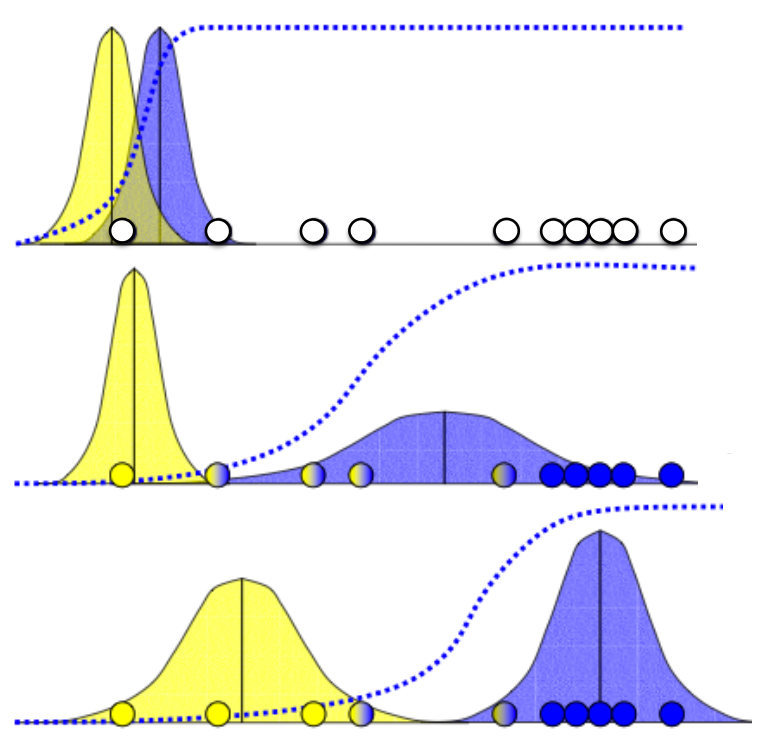
\includegraphics[width=1\linewidth]{1-d.png}
    \caption{}
    \label{ris:experimcoded}
    \end{center}
    \end{figure}

    Оценка этих параметров была бы тривиальной, если бы мы знали, какому из распределений принадлежит каждое из наблюдений:
    $$\mu_a = \frac{x_1 + x_2 + ... + x_{n_a}}{n_a}, \ \ \sigma^2_a = \frac{(x_1 - \mu_a) + (x_2 - \mu_a) + ... + (x_{n_a} - \mu_a)}{n_a}$$
    Аналогично для $(\mu_b, \sigma^2_b)$.

    И, наоборот, зная параметры $(\mu, \sigma^2)$ мы определяем, какова вероятность принадлежности наблюдения этому распределению по формуле Байеса:
    $$ b_i = P(b \mid x_i) = \frac{P(x_i \mid b)P(b)}{P(x_i \mid b)P(b)+P(x_i \mid a)P(a)}, \ a_i = P(a \mid x_i) = 1 - b_i$$
    где $P(x_i \mid b) = \frac{1}{\sqrt{2\pi\sigma^2_b}}e^{-\frac{(x_i-\mu_b)^2}{2\sigma^2_b}}$.

    Следовательно, в нашей задаче необходимо знать параметры $(\mu, \sigma^2)$ для оценки принадлежности наблюдений распределениям и в то же время знать распределение для оценки параметров. Тут и приходит на помощь EM-алгоритм (Рис. 1):
        \begin{enumerate}
        \item
        возьмем случайным образом два гауссовых распределения $(\mu_a, \sigma^2_a)$ и $(\mu_b, \sigma^2_b)$;
        \item
        \textbf{E-шаг:} вычислим $a_i$ и $b_i$ для каждого наблюдения;
        \item
        \textbf{M-шаг:} пересчитываем $(\mu_a, \sigma^2_a)$ и $(\mu_b, \sigma^2_b)$ по формулам:
        $$\mu_a = \frac{a_1x_1 + ... + a_nx_n}{a_1 + ... + a_n}, \ \ \sigma^2_a = \frac{a_1(x_1 - \mu_a) + ... + a_n(x_n - \mu_a)}{a_1 + ... + a_n}$$
        Аналогично для $(\mu_b, \sigma^2_b)$;
        \item
        продолжаем итеративно вплоть до сходимости;
        \end{enumerate}
    Также в M-шаге можно было пересчитывать априорные вероятности $P(b) = \frac{b_1 + ... + b_n}{n}$ и $P(a) = 1 - P(b)$.

    \item

    $m > 1, \ k > 2.$

    $$P(c) = \frac{1}{n} \sum_{i=1}^n P(c \mid  \vec{x_i}) \ \text{для кластера с}$$
    $$\mu_{c, j}=\sum_{i=1}^{n}\left(\frac{P\left(c \mid \vec{x}_{i}\right)}{n P(c)}\right) x_{i, j}$$
    $$\left(\Sigma_{c}\right)_{j, k}=\sum_{i=1}^{n}\left(\frac{P\left(c \mid \vec{x}_{i}\right)}{n P(c)}\right)\left(x_{i, j}-\mu_{c, j}\right)\left(x_{i, k}-\mu_{c, k}\right)$$
    $$P(c \mid \vec{x}_i) = \frac{P(\vec{x_i} \mid c)P(c)}{\sum_{c'=1}^k P(\vec{x_i} \mid c')P(c')}$$
    $$P\left(\vec{x}_{i} \mid c\right)=\frac{1}{\sqrt{2 \pi\left|\Sigma_{c}\right|}} \exp (-\frac{1}{2} \underbrace{\left(\vec{x}_{i}-\vec{\mu}_{c}\right)^{T}\Sigma_{c}^{-1}\left(\vec{x}_{i}-\vec{\mu}_{c}\right))}_{\sum_{j=1}^{d} \sum_{k=1}^{d}\left(x_{i, j}-\mu_{c, j}\right)\left(\Sigma_{c}^{-1}\right)_{j k}\left(x_{i, k}-\mu_{c, k}\right)}$$
    \end{enumerate}



\subsection{Применение EM-алгоритма}

В данной работе EM-алгоритм представлен классом GaussianMixture \cite{fifth}, предложенной библиотекой scikit-learn. Этот класс позволяет оценивать параметры гауссовских распределений.

Метод fit этого класса оценивает параметры модели с помощью EM-алгоритма. Метод fit итерируется между E-шагом и M-шагом указанное количество раз до тех пор, пока изменение правдоподобия или нижней границы не станет меньше некоторого числа. В противном случае возникнет сообщение о том, что метод не сходится.

При создании экземпляра класса указывается количество компонент смеси.

\subsubsection{Проверка работоспособности GaussianMixture}

С помощью модуля stats \cite{sixth} библиотеки Scipy сгенерированы выборки разных распределений.

Для ясности введём следующие обозначения:
\begin{itemize}
    \item cdf --- cumulative distribution function --- функция распределения;
    \item pdf --- probability density function --- плотность вероятности распределения;
    \item std --- standard deviation of the distribution --- среднеквадратическое отклонение распределения.
\end{itemize}

Проверка работоспособности проводится в несколько этапов.

\begin{enumerate}
    \item {
        Напомним формулу гауссовского распределения
        $$ p(x) = \frac{1}{\sqrt{ 2 \pi \sigma^2 }} e^{ - \frac{ (x - \mu)^2 } {2 \sigma^2} },$$

        где параметр $\mu$ --- математическое ожидание и $\sigma$ среднеквадратическое отклонение распределения. Квадрат среднеквадратического отклонения, $\sigma^2$, называется дисперсией.

        Генерирование одного одномерного гауссовского распределения:
        \begin{verbatim}
mu = 0
variance = 1
sigma = math.sqrt(variance)
x = np.linspace(mu - 3*sigma, mu + 3*sigma, 100)
data = norm.pdf(x, mu, sigma)
        \end{verbatim}
        \begin{figure}[h]
            \begin{center}
                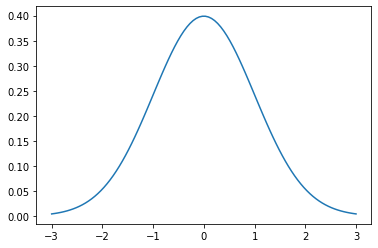
\includegraphics[width=0.7\linewidth]{1-d-gaussian-plot.png}
                \caption{}
                \label{ris:experimcoded}
            \end{center}
        \end{figure}

        Проверка оценки параметров соответствующей выборки с помощью GaussianMixtureModel:
        \begin{verbatim}
k = 1
model = gmm(n_components=k, covariance_type='full')
model.fit(data)
        \end{verbatim}

        Вывод программы:
        \begin{verbatim}
data_mean: 0.1645975096425618
data_covariance: 0.13947206450268224
model_mean: 0.16459751
model_covariance: 0.13947565
        \end{verbatim}

        В результате видим, что оценка параметров GaussianMixtureModel в точности совпадает с реальными параметрами.
    }
    \item {
        Генерирование двух одномерных гауссовских распределений:
        \begin{verbatim}
mu_1 = 2
variance_1 = 4
sigma_1 = math.sqrt(variance_1)

mu_2 = 10
variance_2 = 1
sigma_2 = math.sqrt(variance_2)

x_1 = np.linspace(mu_1 - 3*sigma_1, mu_1 + 3*sigma_1, 100)
x_2 = np.linspace(mu_2 - 3*sigma_2, mu_2 + 3*sigma_2, 100)
data_1 = norm.pdf(x_1, mu_1, sigma_1)
data_2 = norm.pdf(x_2, mu_2, sigma_2)
        \end{verbatim}
        \begin{figure}[h]
            \begin{center}
                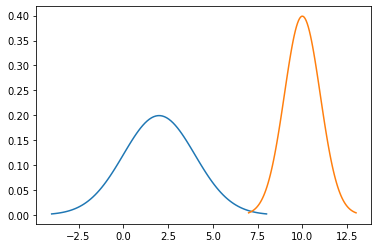
\includegraphics[width=0.7\linewidth]{1-d-gaussuans-plot.png}
                \caption{}
                \label{ris:experimcoded}
            \end{center}
        \end{figure}

        Генерирование одной выборки для двух распределений и проверка оценки её параметров с помощью GaussianMixtureModel:
        \begin{verbatim}
new_data = np.concatenate((data_1, data_2), axis=0)
np.random.shuffle(new_data)

k = 2
model = gmm(n_components=k,
            max_iter=1000,
            covariance_type='full')
model.fit(new_data)
        \end{verbatim}
        Вывод программы:
        \begin{verbatim}
data_mean_1: 0.0822987548212809
data_covariance_1: 0.06973603225134112
data_mean_2: 0.16459750964256176
data_covariance_2: 0.1394720645026822

model_mean_1: 0.01832714
model_covariance_1: 0.01409637
model_mean_2: 0.18062076
model_covariance_2: 0.10954001
        \end{verbatim}
        Здесь во время многократных экспериментов точность результата варьировалась в зависимости от исходных распределений.
    }
    \item {
        Генерирование одного двумерного гауссовского распределения:

        \begin{verbatim}
x = np.linspace(0, 10, 100)
y = np.linspace(10, 20, 100)
X, Y = np.meshgrid(x, y)

mu_x = np.mean(x)
sigma_x = np.std(x)
mu_y = np.mean(y)
sigma_y = np.std(y)
norm = multivariate_normal([mu_x, mu_y],
                           [[sigma_x, 0], [0, sigma_y]])

pos = np.empty(X.shape + (2,))
pos[:, :, 0] = X
pos[:, :, 1] = Y
data = norm.pdf(pos)
        \end{verbatim}
        \begin{figure}[h]
            \begin{center}
                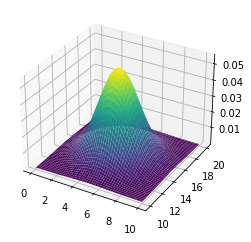
\includegraphics[width=0.5\linewidth]{2-d-gaussian-plot.png}
                \caption{}
                \label{ris:experimcoded}
            \end{center}
        \end{figure}

        Проверка оценки параметров соответствующей выборки с помощью GaussianMixtureModel:
        \begin{verbatim}
k = 2
model = gmm(n_components=k,
            max_iter=10000,
            covariance_type='full')
model.fit(new_data)
        \end{verbatim}

        Вывод программы:
        \begin{verbatim}
data_mean_x: 5.0
data_covariance_x: 2.9157646512850626
data_mean_y: 15.0
data_covariance_y: 2.9157646512850626

model_mean_x: 5.12451189
model_covariance_x: 3.16980297
model_mean_y: 14.7726552
model_covariance_y: 3.22703713
        \end{verbatim}

        Здесь во время многократных экспериментов точность результата варьировалась в зависимости от исходных распределений.
    }
    \item {
        Напомним формулу равномерного распределения
        $$p(x) = \frac{1}{b - a},$$
        принимающая значения $p(x)$ в промежутке $[a, b)$, и ноль --- вне промежутка.

        Генерирование одного одномерного равномерного распределения:
        \begin{verbatim}
a = 0
b = 5
size = 100
uni = uniform(loc=a, scale=b)
x = np.linspace(uni.ppf(0), uni.ppf(1), size)
data = uni.pdf(x)

        \begin{figure}[h]
            \begin{center}
                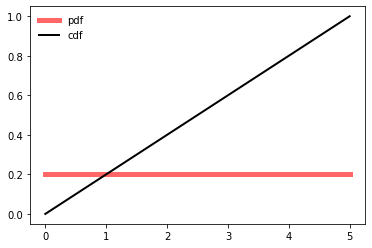
\includegraphics[width=0.5\linewidth]{1-d-uniform-plot.png}
                \caption{}
                \label{ris:experimcoded}
            \end{center}
        \end{figure}
        \end{verbatim}

        Проверка оценки параметров соответствующей выборки с помощью GaussianMixtureModel:
        \begin{verbatim}
k = 1
model = gmm(n_components=k, covariance_type='full')
model.fit(data)
        \end{verbatim}

        Вывод программы:
        \begin{verbatim}
data_mean: 0.19999999999999996
data_covariance: 5.551115123125783e-17
model_mean: 0.2
model_covariance: 0.001
        \end{verbatim}

        В результате видим, что оценка параметров равномерной выборки с помощью GaussianMixtureModel далека от истинного значения.
    }
\end{enumerate}

\subsubsection{Применение EM-алгоритма к цензурированной выборке}

Дана выборка объема $n = 97$ вида $\{(z_{(i)}, \delta_{(i)}),\ i=\overline{1,n}\}$:

(777;1), (781;0), (843;0), (866;0), (869;1), (872;1), (876;1), (893;1), (894;1), (895;0), (898;1), (906;0), (907;1), (909;1), (911;1), (911;0), (914;0), (927;1), (932;1), (936;0), (940;0), (942,5;0), (943;0), (945;1), (945;0), (948;1), (951;0), (953;0), (956;0), (957;1), (957;0), (959;0), (960;0), (966;1), (966;0), (969;1), (970;0), (971;1), (972;0), (973;0), (977;0), (983;1), (984;0), (985;1), (989;1), (992,5;1), (993;1), (996;1), (998;1), (1001;0), (1002;0), (1005;0), (1006;0), (1009;1), (1011,5;1), (1012;1), (1012;0), (1013;0), (1015;0), (1016;0), (1018;0), (1022;1), (1023;0), (1025;1), (1027;0), (1029;1), (1031;1), (1031;0), (1031,5;0), (1033;1), (1036;1), (1043;1), (1043;0), (1044;1), (1044;0), (1045;0), (1047;0), (1053;1), (1055;1), (1058;0), (1059;1), (1060;1), (1060;0), (1064;0), (1070;0), (1073;0), (1080;1), (1085;1), (1093;0), (1093,5;1), (1094;1), (1106;0), (1107;0), (1118;0), (1128;1), (1139;1), (1153;0).

\begin{figure}[h]
    \begin{center}
        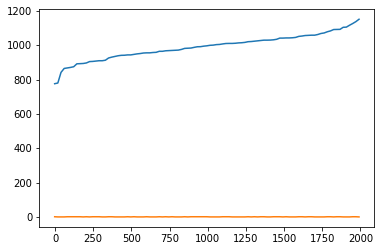
\includegraphics[width=0.7\linewidth]{lab-data-plot.png}
        \caption{}
        \label{ris:experimcoded}
    \end{center}
\end{figure}

Данные представлены в месяцах, причем число 1 в парах означает нецензурирование (т.е. смерть), а 0 - цензурирование. При этом 46 человек умерли с начала открытия центра в 1964 году по 1 июля 1975 года ко дню сбора данных. Это нецензурированные данные. Из остальных 51 человек 5 были выписаны из центра, а 46 ещё были живы к 1 июля 1975 года. Это цензурировананные данные.

Построим следующую оценку по формулам:
\begin{multline*}
    F_n^{RR}(x) = 1 - (1 - H_n(x))^{\frac{\Lambda_{1n}(x)}{\Lambda_n(x)}} = \\ = \left\{ \begin{array}{cl} 0, & x < z_{(1)} \\ 1 - (1 - \frac{k}{n})^{\frac{\Lambda_{1n}(x)}{\Lambda_n(x)}}, & z_{(k)} \le x < z_{(k+1)}, k = \overline{1,n} \\ 1, & x \ge z_{(n)} \end{array} \right.,
\end{multline*}
где
\[
    1 - H_n(x) = \frac{1}{n} \sum_{j=1}^n I(z_{(j)} > x),
\]
\begin{multline*}
    \Lambda_{1n}(x) = \int_{-\infty}^x \frac{dH_{1n}(u)}{1 - H_{1n}(u-)} = \\ = \frac{1}{n} \sum_{j=1}^n \frac{\delta_{(j)} I(z_{(j)} \le x)}{\frac{1}{n} \sum_{i=1}^n I(z_{(i)} \ge z_{(j)})} = \sum_{j=1}^n \frac{\delta_{(j)} I(z_{(j)} \le x)}{\sum_{i=1}^n I(z_{(i)} \ge z_{(j)})},
\end{multline*}
\[
    \Lambda_{n}(x) = \int_{-\infty}^x \frac{dH_n(u)}{1 - H_n(u-)} = \sum_{j=1}^n \frac{I(z_{(j)} \le x)}{\sum_{i=1}^n I(z_{(i)} \ge z_{(j)})}.
\]

Приведём код программы, которая реализует вышеизложенные формулы и строит оценку $F_n^{RR}$.
\begin{verbatim}
def one_minus_H_n(x, data):
    n = len(data)
    result = 0
    for i in range(n):
        result += 1 if data[i][0] > x else 0
    result /= n
    return result

def Lambda_1n(x, data):
    n = len(data)
    result = 0
    numerator = 0
    denominator = 0
    for i in range(n):
        denominator = 0
        numerator = data[i][1] * (1 if data[i][0] <= x else 0)
        for j in range(n):
            denominator += (1 if data[j][0] >= data[i][0] else 0)
        result += numerator / denominator
    return result

def Lambda_n(x, data):
    n = len(data)
    result = 0
    numerator = 0
    denominator = 0
    for i in range(n):
        denominator = 0
        numerator = 1 if data[i][0] <= x else 0
        for j in range(n):
            denominator += (1 if data[j][0] >= data[i][0] else 0)
        result += numerator / denominator
    return result

def FnRR(x, data):
    result = 1 - one_minus_H_n(x, data)**(Lambda_1n(x, data) /
                                            Lambda_n(x, data))
    return result
\end{verbatim}

\begin{figure}[h]
    \begin{center}
        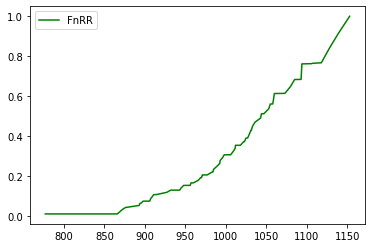
\includegraphics[width=0.7\linewidth]{FnRR.png}
        \caption{}
        \label{ris:experimcoded}
    \end{center}
\end{figure}

По следующим формулам вычислим математическое ожидание и дисперсию для цензурированной выборки:

$$\hat{\mu}_n = \int_{z(1)}^{z(n)} tdF_n^{RR} (t) = \sum_{i=1}^{n} z_{(i)} \Delta F_n^{RR} (z_i) $$
$$\hat{\sigma}_n^2 = \int_{z(1)}^{z(n)} (t - \hat{\mu}_n)^2 dF_n^{RR} (t) = \sum_{i=1}^{n} (z_{(i)} - \hat{\mu}_n)^2 \Delta F_n^{RR} (z_i),$$
где $\Delta F_n^{RR} (z_i)$ --- скачок функции.

Приведём код программы, которая реализует вышеизложенные формулы в одной функции:
\begin{verbatim}
def calculate_mu_and_sigma(z, data):
n = len(data)
mu = z[0] * FnRR(z[0], data)
for i in range(2, n):
    mu += z[i] * (FnRR(z[i], data) - FnRR(z[i-1], data))
variance = (z[0] - mu) ** 2 * FnRR(z[0], data)
for i in range(2, n):
    variance += (z[i] - mu) ** 2 * (FnRR(z[i], data)
                                    - FnRR(z[i-1], data))
sigma = sqrt(variance)
return mu, sigma
\end{verbatim}

\newpage

\section{Заключение}
    В данной работе было собрано методическое пособие по знакомству с EM-алгоритмом на примере смеси гауссовых распределений. Было дано описание самого алгоритма, которое позволит быстро ознакомиться с его теоретической частью.
    
    Также был выполнен следующий прикладной вклад. Во-первых, былоа наглядно продемонстрирована генерация выборок разных распределений и исследованы результаты способностей GaussianMixture оценивать параметры таких выборок. Во-вторых, был сделан новый шаг по вычислению математического ожидания и дисперсии цензурированных выборок на основе оценки функции распределения таких выборок $F_n^{RR}$, предложенной Абдушукуровым А. А., и был применён EM-алгоритм к реальным цензурированным данным.
    
    В дальнейшем предполагается увеличение компонент смеси распределений и расширение семейства самих распределений, подаваемых на вход EM-алгоритму. К примеру, разработка GeneralMixture, позволяющей оценивать параметры любого семейства распределений.
    
    Автор выражает благодарность Абдушукурову А. А. за научное руководство.
\newpage

\begin{thebibliography}{99}

\bibitem{first} Dempster A. P., Laird N. M., Rubin D. B. Maximum likelihood from incomplete data via the EM algorithm // J. of the Royal Statistical Society, Series B. — 1977. —no. 34. — Pp. 1–38.

\bibitem{second} Шлезингер М. И. О самопроизвольном различении образов // Читающие автоматы. — Киев, Наукова думка, 1965. — Pp. 38–45

\bibitem{third} Айвазян С. А., Бухштабер В. М., Енюков И. С., Мешалкин Л. Д. Прикладная статистика: классификация и снижение размерности. — М.: Финансы и статистика, 19

\bibitem{fourth} В. Ю. Королёв. ЕМ-алгоритм, его модификации и их применение к задаче разделения смесей вероятностных рспределений

\bibitem{fifth} Документация GaussianMixture \\ \url{https://scikit-learn.org/stable/modules/generated/sklearn.mixture.GaussianMixture.html#sklearn.mixture.GaussianMixture}

\bibitem{sixth} Документация к модулю stats библиотеки Scipy \\ https://docs.scipy.org/doc/scipy/reference/tutorial/stats.html

\end{thebibliography}

\end{document}